\pdfoutput=1

\documentclass[11pt]{article}
\usepackage{graphicx}

% Remove the "review" option to generate the final version.
\usepackage[final]{ACL2023}

% Standard package includes
\usepackage{times}
\usepackage{latexsym}

% For proper rendering and hyphenation of words containing Latin characters (including in bib files)
\usepackage[T1]{fontenc}

% This assumes your files are encoded as UTF8
\usepackage[utf8]{inputenc}

% This is not strictly necessary, and may be commented out.
% However, it will improve the layout of the manuscript,
% and will typically save some space.
\usepackage{microtype}

% This is also not strictly necessary, and may be commented out.
% However, it will improve the aesthetics of text in
% the typewriter font.
\usepackage{inconsolata}

% useful for filling with text
\usepackage{lipsum}
%\setcitestyle{numbers}



% title should maybe be shortened but its good for now.
% Analyzing RALMs with Selective State Space and Attention based Models for Long Sequence
\title{Analyzing RALMs with Selective State Space and Attention based Architectures for Long Sequence Modeling}

\author{Sebastian P. Jaskowski$^1$ \and Nolan M. Bridges$^1$ \and Austin T. Barton$^1$ \\
        \\
         $^1$Georgia Institute of Technology \\ 
         \\ 
         \texttt{sjaskowski3@gatech.edu} \\ \texttt{bridges@gatech.edu} \\
         \texttt{abarton40@gatech.edu} \\}

\begin{document}
\maketitle

\section{Introduction}
Recently, a new language model paradigm has emerged in the form of Retrieval Augmented Language Models, or RALMs \cite{lewis2021retrievalaugmented, gao2024retrievalaugmented}. These models improve upon stand-alone language models by utilizing a retriever to acquire and inject relevant context information into a language model prompt during inference time. By injecting knowledge into the model at runtime, this paradigm addresses limitations such as outdated parameterized knowledge, the generation of false or incorrect statements, and the lack of supportive reasoning for responses. 

Most recent language models, and thus almost all Retrieval Augmented Language Models, have been built upon the transformer architecture. \cite{vaswani2023attention}. While the transformer has allowed for incredibly powerful language models due to its ability to selectively learn relationships between arbitrary elements in sequential data, it also introduces drawbacks such as quadratic scaling over sequence length, resulting in limited context windows \cite{xu2024retrieval}, and difficulty considering all information within its context window even when the information fits. \cite{liu2023lost}. These limitations of transformer-based models are particularly impactful on RALMs, as they effectively place an upper-limit on the number of retrieved context chunks a RALM can process.

On a different note, recent work in the field of state space models (SSMs), most notably in the form of the newly proposed Mamba architecture, has shown strong results on sequence modelling tasks, especially on long sequences with Long Range Dependencies, or LRDs \cite{gu2022, gu2021combining}. This new architecture holds promising potential for its use as a language model for RALMs, due to its ability to process and utilize a higher number of retrieved chunks, potentially leading to higher accuracy on QA tasks. Specifically, it may see higher performance when there are more retrieved chunks to parse through, due to its demonstrated stronger ability at signal/noise disambiguation.

\begin{figure}[t]
    \centering
    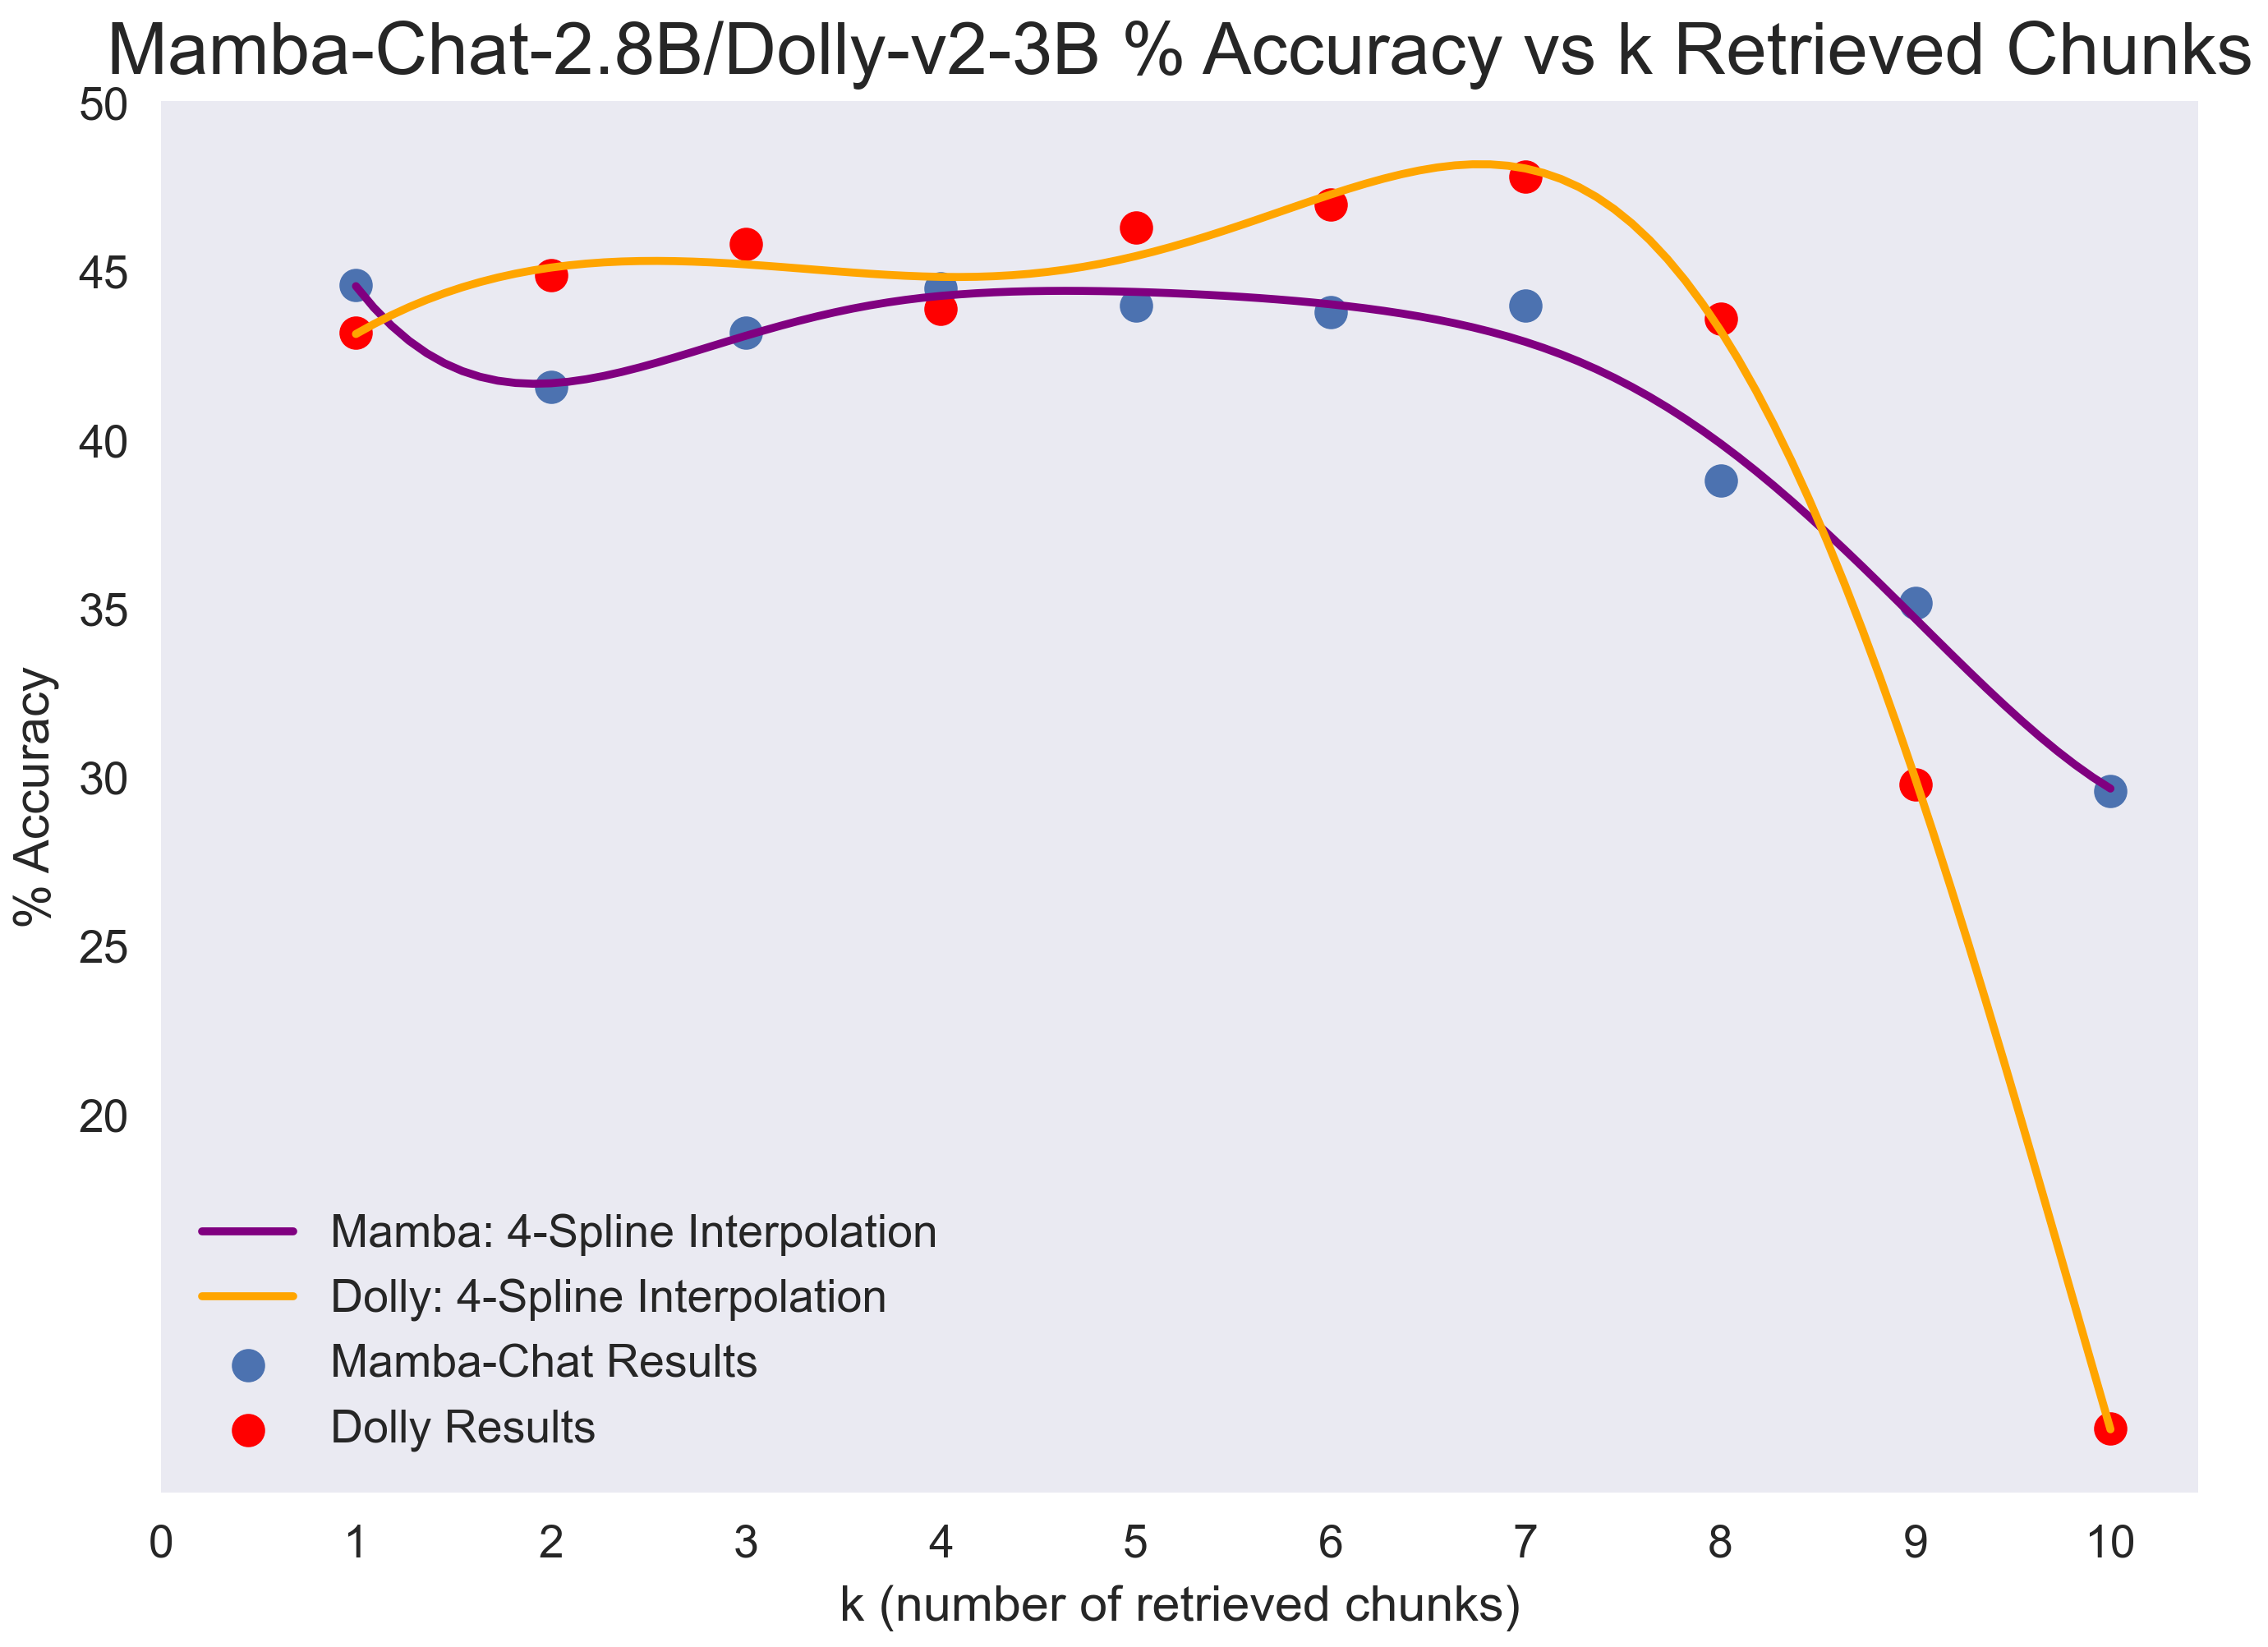
\includegraphics[width=0.49\textwidth]{rag-results-over-k.png}
    \caption{Scatter plot of accuracy results of Mamba-Chat-2.8B and Dolly-v2-3B over each $k$ value with $B$-Spline ($B=4$) interpolation.}
    \label{fig:mamba-chat-results}
\end{figure}

As such, we aim to assess these claims by providing the first comprehensive, end-to-end evaluation and benchmarking of a RALM constructed upon a language model based on the Mamba architecture. We construct a RALM based on the 2.8B parameter instruction-tuned Mamba-Chat model \cite{haven2023mambachat} and evaluate it on a subset of the popular QA benchmarking dataset TriviaQA \cite{Joshi2017TriviaQAAL}. We compare our results to the performance of a RALM based on the 2.8B parameter instruction-tuned Dolly-v2-3b model \cite{DatabricksBlog2023DollyV2}, and we evaluate both models over $k$ values ranging from $1$ to $10$ (where $k$ refers to the number of context chunks retrieved from the vector database and fed to the language model).

We find that both models see similar performance for small to medium values of $k$ ($k \leq 7)$, and the performance of both models declines as $k$ grows. This contradicts our initial assumption that the Mamba-Chat model would see a significant, overall performance increase when compared to Dolly-v2-3b. However, when large amounts of context are presented ($k > 7$), we see that the performance degradation faced by Dolly-v2-3b is much greater than that faced by the Mamba-Chat model. This suggests that Mamba-Chat may be more resilient to the larger amounts of irrelevant information present when $k$ is larger.
 
\section{Background}
\subsection{Retrieval-Augmented Language Models}
For the past few years, Large Language Models (LLMs) have dominated the field of Natural Language Processing (NLP) due to their ability to function as Few-Shot Learners \cite{brown2020language}, achieving state of the art performance on a variety of NLP tasks without task-specific training. However, key limitations remain, such as their inability to update their parameterized knowledge base to incorporate new information, their tendency to produce made-up information (a behavior that has been referred to as "hallucinations"), and their inability to source their information, which reduces user trust in the model. \cite{lewis2021retrievalaugmented, huang2023survey}. 

As a result, RALMs emerged as a effective solution to address these drawbacks by providing an external non-parametric knowledge base in the form of a vector index, from which a the model can retrieve relevant knowledge context that can then be appended to the initial prompt \cite{lewis2021retrievalaugmented}. By having relevant knowledge in the prompt, the LLM no longer relies on its parametric knowledge, which is often inaccurate and leads to the common problems described above.

Retrieval-augmented models operate in a multi-step process. Before inference, a large corpus of text that contains potentially relevant information to future prompts is chunked, embedded using an embedding model, and stored in a vector database that maps vector representations to their corresponding chunks. At inference time, the query to the model is embedded using the same embedding model as used during database creation, and the $k$ most relevant chunks (where $k$ is a hyperparameter), as determined by cosine similarity of embeddings, is retrieved. These chunks are then combined with the original query to form a language model prompt, which is passed to the LLM. 

\begin{figure}[t]
    \centering
    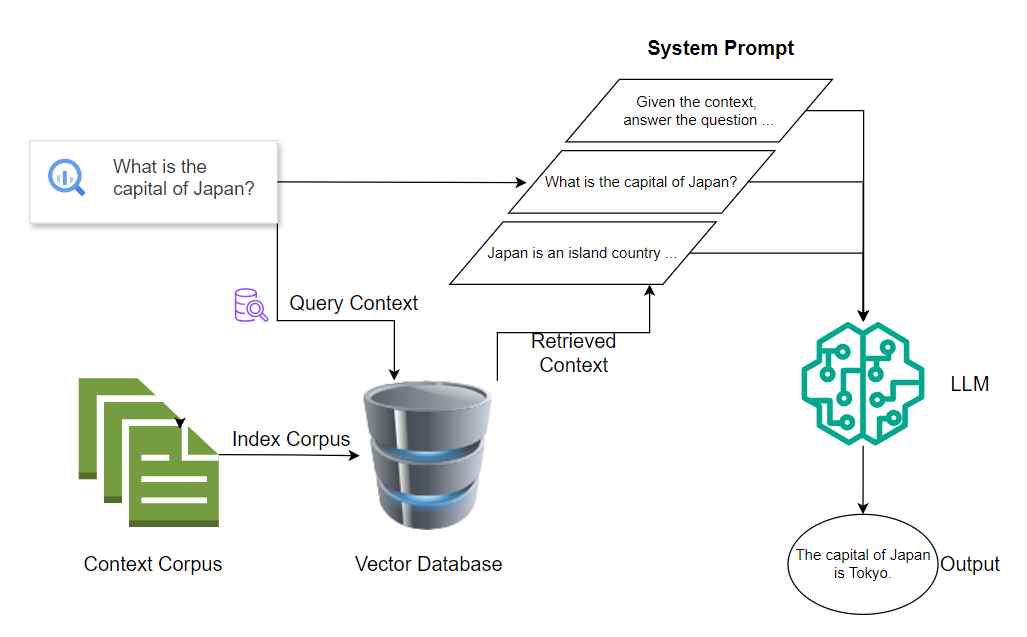
\includegraphics[width=1\linewidth]{overleaf/rag_diagram.png}
    \caption{Diagram of standard Retrieval-Augmented Language Model}
    \label{fig:enter-label}
\end{figure}

While RALMs have found tremendous success in QA tasks, recent studies have highlighted that transformer-based Retrieval-Augmented Language Models (RALMs) face significant challenges when handling extensive amounts of retrieved knowledge. The inherent quadratic memory constraints of the self-attention mechanism limit the context window, which in turn poses difficulties in integrating sufficient context. This limitation has spurred investigations into various information condensation strategies, including PRCA \cite{yang-etal-2023-prca}, RECOMP \cite{xu2023recomp}, and the Filter-Reranker approach \cite{ma2023large}. Furthermore, evidence from recent research suggests that even as the context windows are enlarged in more substantial models, transformer language models exhibit limitations in effectively leveraging all pertinent content chunks \cite{xu2024retrieval} \cite{liu2023lost}. 

\subsection{State Space Models}

These challenges have a potential solution in State Space Models, or SSMs. While research into SSMs fell out of the limelight due to the prominent success of the transformer architectures, State Space Models promise a key significant improvement over transformers in the form of linear scaling over sequence length, as opposed to the quadratic scaling found in transformers. In 2021, researchers developed the Linear State Space Layer (LSSL), a model that combines linear recurrence with a continuous-time state space \cite{gu2021combining}. This model was further improved upon by Structured State Space Models, commonly referred to as S4, which alleviated the heavy computational requirements that previously hindered LSSLs \cite{gu2022}. These models saw great performance improvements over previous state-of-the-art, yet still struggled to match the performance and efficiency of Transformers on language tasks \cite{gu2023mamba}.

More recently, the Mamba architecture emerged. This variation of the S4 model saw an added selectivity mechanism, allowing the model to become context-aware and selectively consider specific sequence elements while maintaining fast computation and efficient memory usage. This improvement ended up being crucial to boosting the performance of State Space Models; Mamba achieved state-of-the-art performance on sequences up to 1M tokens, and 5 times faster inference than similarly sized transformers \cite{gu2023mamba}.

\section{Methodology}
We construct our RALM models using a common Retrieval-Augmented Generation (RAG) framework for all language model architectures, ensuring that the only difference between RALMs is the underlying language model. All models utilize the same retriever, vector index, and prompting format.
\subsection{Vector Index}
To support efficient and accurate context retrieval, we constructed our vector database using the Facebook AI Similarity Search (FAISS) vector database \cite{johnson2017billionscale}. 
We began by aggregating 10,031 wikipedia articles designated as ground truth context in the TriviaQA dataset \cite{Joshi2017TriviaQAAL}. This set of articles is a subset of a larger context base of 73,976 wikipedia articles, however we removed all articles that were not designated as a ground truth reference by any question in our QA dataset in order to alleviate the prohibitively expensive computational requirements of embedding such a high amount of text.

These 10,031 wikipedia articles, totalling 223MB of data, were then chunked (with chunk size equal to 1000 characters) and passed through the \textit{bge-small-en-v1.5} embedding model \cite{bge_embedding} to create vector representations of chunks. Context embedding remains a computational bottleneck for RALMs; thus, our choices of chunk size and embedding model reflect this limitation. We chose the \textit{bge-small-en-v1.5} embedding model due to its small size of only 0.13GB and relatively high performance. We set our target chunk size at 1000\footnote{While we set our target chunk size to 1000, chunk lengths vary due to long sequences of consecutive characters without the occurrence of our split character (a newline character).} as smaller chunk sizes would have resulted in prohibitively expensive chunking and embedding time.

Upon completion of indexing, the original 10,031 wikipedia articles resulted in 245,624 chunks stored in our vector database.
\subsection{Retriever}
To perform retrieval, we utilized the FAISS library to perform efficient k-Nearest Neighbors search based on cosine similarity over our vector database. We chose to utilize the FAISS library due to its efficient utilization of GPUs when performing similarity search, which significantly sped up RALM inference \cite{johnson2017billionscale}.
\subsection{Prompt Formatting}
To ensure maximum fairness in evaluation, we standardized our prompt across all models evaluated. Our prompt was constructed based on careful review of previously used system prompts for Retrieval-Augmented Language Models.
\newline
\newline
Our prompt is displayed below.
\begin{quote}
    \textit{Please respond to the original query. If the selected document context is relevant and informative, provide a detailed answer based on its content. However, if the selected document context does not offer useful information or is not applicable, simply state 'No answer found'}
\end{quote}
\subsection{Language Models}
We evaluate two language models within our Retrieval-Augmented Generation structure: the 2.8B parameter instruction-tuned Mamba-Chat model based on the Mamba architecture and the 2.8B parameter instruction-tuned Dolly-v2-3b model based on the transformer architecture.
\begin{table}[t]
    \centering
    \begin{tabular}{|c|c|c|} 
     \hline
     \textbf{Model} & Mamba-Chat & Dolly-v2-3b \\
     \hline\hline
     Num. Parameters & 2.8B & 2.8B \\ 
     \hline
     Context Limit & unlimited & 2048 tokens \\
     \hline
     Instruction-tuned? & Yes & Yes \\
     \hline
     Temperature & 0 & 0 \\
     \hline
    \end{tabular}
    \caption{Comparison of Models Evaluated}
    \label{tab:my_label}
\end{table}

We chose the Mamba-Chat model as it was one of few existing instruction-tuned language models based on the Mamba architecture. We then chose Dolly-v2-3b as our baseline transformer model due to its relatively-decent success, and comparable model size to Mamba-Chat. 
\subsection{Inference and Evaluation Methodology}
In order to assess the ability of our RALMs, we evaluate the models over a subset of the popular Question-Answering (QA) benchmark TriviaQA \cite{Joshi2017TriviaQAAL}. This dataset features a set of questions, with each question matched to a particular noun answer, as well as a list of possible aliases for that answer.

Due to an average model inference time in excess of 10 seconds, evaluating over the entire dataset is beyond the capabilities of our computational resources. As such, we chose to evaluate our models over a random sample of 1,000 questions from the TriviaQA dataset.

Both models were evaluated with varying amounts of retrieved context, with $k$ ranging from 1 to 10. An upper-bound at 10 was chosen to due increasing evaluation times at higher values of $k$ (due to greater execution time of Nearest Neighbor Search in retrieval), as well as context window limitations on Dolly-v2-3b. We then perform an additional evaluation on Mamba-Chat at $k=20$, yet this result is incomparable since $k=20$ would far exceed the context length on Dolly-v2-3B.

To evaluate whether a given model-generated answer is correct, we checked if any alias of the correct answer appeared in the model output text. We refer to this evaluation approach as Exact Subsequence Matching. Due to the nature of this dataset featuring answers that are proper nouns, we believed that this evaluation methodology accurately reflects the performance of this model in this particular QA task.

Evaluations were performed on a High-RAM Google Colab instance utilizing a T4 GPU.
\section{Results}
We find that both Mamba-Chat and Dolly-v2-3b perform similarly for small to medium amounts of retrieved context, and while both models encounter performance degradation as $k$ increases, the Mamba-Chat model remains more resilient to these declines in performance. Our results are summarized in Table 2 and visualized in Figure 1.

For small to medium values of $k$, we find that both models achieve similar performance, with Dolly-v2-3b slightly outperforming its counterpart. This contradicts our initial assumption that Mamba-Chat would see overall greater performance. We acknowledge that the performance for small and medium values of $k$ is likely bottle-necked by the retrieval process, and the use of a more powerful embedding model may lead to higher performance overall, as well as the occurrence of a performance disparity at higher accuracy levels.

As $k$ grows to larger values, we see that the performance of both models begins to decline, with the performance of Dolly-v2-3B declining significantly greater than that of Mamba-Chat. At $k=10$, we find that Mamba-Chat achieves an Exact Subsequence Match accuracy of $29.6\%$, while Dolly-v2-3B achieves only $10.7\%$.
\begin{table}[t]
    \centering
    \begin{tabular}{|c|c|c|} 
     \hline
     \textbf{Model} & Mamba-Chat & Dolly-v2-3b \\
     \hline\hline
     k=1 & 44.6\% & 43.2\% \\ 
     \hline
     k=2 & 41.6\% & 44.9\% \\
     \hline
     k=3 & 43.2\% & 45.8\% \\
     \hline
     k=4 & 44.5\% & 43.9\% \\
     \hline
     k=5 & 44.0\% & 46.3\% \\
     \hline
     k=6 & 43.8\% & 47.0\% \\
     \hline
     k=7 & 44.0\% & 47.8\% \\
     \hline
     k=8 & 38.8\% & 43.6\% \\
     \hline
     k=9 & 35.2\% & 29.8\% \\
     \hline
     k=10 & 29.6\% & 10.7\% \\
     \hline
     \hline
     k=20 & 21.5\% & N/A \\
     \hline
    \end{tabular}
    \caption{Accuracy of Models on TriviaQA dataset-subset.}
    \label{tab:my_label}
\end{table}

We infer that this performance decline is caused by two factors: (1) context window limitations in the transformer-based model and (2) model's inability to effectively consider all context in its input. 

The former of these is only applicable to Dolly-v2-3b, as the nature of the Mamba architecture does not necessitate an explicit context length. Our maximum $k$ value of 10 was chosen such that model input did not exceed 2048 tokens\footnote{This is based on an assumption of 5 characters per token, resulting in 200 tokens per context chunk, which means 2000 tokens of total context at $k=10$}, but due to variations in tokenization and chunking, we cannot guarantee that prompts did not exceed the context window length of Dolly-v2-3b. This leads us to conclude that context window length limitations may have been a factor in the sudden decrease in performance of Dolly-v2-3b at larger values of $k$.

The second potential factor for performance decreases in both models is the ability of the model to properly utilize all inputted context chunks. Due to previous work demonstrating the strong performance of the Mamba architecture on modeling Long Range Dependencies \cite{gu2023mamba}, we believed that Mamba-Chat would continue to be performant as inputted context lengths increased. Our results show that while performance reduction in Mamba-Chat as $k \to 10$ does occur, it is not as significant as that seen in Dolly-v2-3b. This leads us to confirm our initial hypothesis: Mamba-Chat does demonstrate stronger resilience to increased context input than transformer-based models. This is particularly evident with Mamba-Chat maintaining an Exact Subsequence Match accuracy of 21.5\% at $k=20$, while the accuracy of Dolly-v2-3b falls to 10.7\% by $k=10$. 
\section{Conclusion}
In this work, we aimed to perform a comprehensive, end-to-end evaluation of the Mamba architecture as a language model for RALM systems, comparing it to the traditional transformer-language model. We evaluate both models on a long-context QA task, utilizing the popular TriviaQA QA evaluation dataset. We find that the Mamba-Chat model does not perform better than a traditional transformer-based language model at low to medium amounts of retrieved context. However, it maintains significantly higher performance, as compared to Dolly-v2-3b, when the amount of retrieved context is high. While both models suffer from performance degradation, Mamba-Chat appears to be significantly more resilient to this degradation.
\section{Limitations and Future Work}
While we aimed to provide a full comprehensive evaluation of differences between our two RALMs, our limited computational resources resulted in some limitations, most notably in the following areas:
\begin{enumerate}
    \item \textbf{Small Number of Evaluated Models.} Due to computational challenges and time constraints, we were only able to compare the Mamba-based RALM to one Transformer-based RALM. There is significant room for future work in comparing the Mamba RALM model to other transformer models, including even models with larger numbers of parameters such 7B parameter models and 13B parameter models, as well as models with larger context length limitations, allowing for evaluation on higher values of $k$.
    \item \textbf{Limited Evaluation Dataset.} Once again due to computational resource constraints, we were only able to benchmark the models on a small subset of the TriviaQA dataset. In future work, we would be interested in performing a more comprehensive evaluation against the entire dataset, as well as expanding the evaluation to other prominent QA benchmarks such as Natural Questions QA \cite{kwiatkowski-etal-2019-natural}.
    \item \textbf{Small Encoding Model} While the embedding model we chose, \textit{bge-small-en-v1.5}, is a high performant model given its size, there are higher performing embedding models available. Unfortunately, we were unable to utilize them due to computational constraints, as larger models would have required more memory usage and embedding time.
\end{enumerate}
In summary, future work in this direction could focus on expanding our evaluation to more transformer-based models, as well as expanding the evaluation to new QA datasets. In particular, future work that attempts to expand our evaluations to larger transformer models with longer context lengths may significantly strengthen the significance of our results.
\clearpage
% Entries for the entire Anthology, followed by custom entries
\bibliography{ref_report}
\bibliographystyle{acl_natbib}
\clearpage
\twocolumn[
\section*{Appendix A}
\appendix{}
\section{Summary of Individual Contributions}
The following table summarizes the specific contributions to the project by individual authors.
\newline
]
\begin{table}[h]
    \centering
    \begin{tabular}{|c|c|c|c|} 
     \hline
     Task & Sebastian Jaskowski & Nolan Bridges & Austin Barton \\
     \hline
     \hline
     Proposal Writing  &25\% & 5\% & 70\% \\
     \hline
     Model Code & 10\% & 70\% & 20\% \\
     \hline
     RAG Framework Code & 20\% & 40\% & 40\% \\
     \hline
     TriviaQA Dataset Preprocessing & 60\% & 30\% & 10\%\\
     \hline
     Evidence Embedding/Vector Index Construction & 60\% & 20\% & 20\%\\
     \hline
     Model Evaluation & 50\% & 10\% & 40\%\\
     \hline
     Final Report Writing & 70\% & 10\% & 20\% \\
     \hline
     Presentation Slides & -- & -- & --\\
     \hline
    \end{tabular}
\end{table}
%This is a section in the appendix.

\end{document}
